\chapter{My contribution}
\label{cha:MyContribution}

This chapter focuses on the implementation of a new segmentation approach by taking the existing methods as reference (see chapter \ref{cha:relatedWork}). The goal is to segment an articulated object into its unknown number \textit{n} of rigid parts \textit{P = \{{part\textsubscript{0}, ...,  part\textsubscript{n}\}}}, which is done by registering the points clouds \textit{S\textsubscript{0}} and \textit{D\textsubscript{0}} of two different poses of the object. Thereby, the algorithm takes advantage of the knowledge that the points located on one rigid part have the same transformation \textit{T = \{T\textsubscript{0}, ...,  T\textsubscript{n}\}}. Basically, a divide and conquer approach is implemented to reduce the computation steps of the correlated correspondence algorithm \cite{Anguelov04}. Furthermore, the LRP approach \cite{correspondence} is employed as an initial registration step to align the two poses of the object. 

\section{Assumptions}

\section{Challenges/restrictions}

There are many challenges regarding the non-rigid registration of point clouds in 2D, as well as in 3D. First off, the input data can be noisy by means of points not belonging to the object. Furthermore, the approach is computationally expensive and time-consuming, as the corresponding body parts of two meshes need to be detected iteratively. Additionally, the inevitable difficulty of finding the global optimum, related to ambiguous body parts, has to be overcome.

\section{Divide and conquer approach}

The point clouds \textit{S\textsubscript{0}} and \textit{D\textsubscript{0}} are iteratively subdivided into point clusters \textit{C = \{{cluster\textsubscript{0}, ...,  cluster\textsubscript{m}\}}}. In each iteration step two related clusters are matched with the ICP (iteratest clostest point) and checked for the total error. In case of a low error, the parts are assumed to match and by dividing them at another part, it is checked, where to segment the part from the other points. For this a divider \textit{d} is used.

\subsection{Basic functionality}

Assuming that the object is only composed of two rigid parts, the approach would work the following:

 The algorithm starts with two sets of point clouds \textit{S\textsubscript{0}} and \textit{D\textsubscript{0}} of the same object in different configurations. The objects are composed of two rigid parts. \textit{S\textsubscript{0}} is used as a \textit{template} to be registered with \textit{D\textsubscript{0}}. The goal is to find a part assignment \textit{P = \{{part\textsubscript{0}, part\textsubscript{1}\}}} and transformation \textit{T = \{T\textsubscript{0}, T\textsubscript{1}\}} for all points of the \textit{template} that alligns them with all points of \textit{D\textsubscript{0}}. To iteratively find corresponding parts and transformations, \textit{S\textsubscript{0}} as well as \textit{D\textsubscript{0}} are divided into clusters \textit{C = \{{cluster\textsubscript{0}, cluster\textsubscript{1}\}}} . The dividers \textit{d\textsubscript{S}} and \textit{d\textsubscript{D}} are initially defined with the secondary axis \textit{s\textsubscript{S}} and \textit{s\textsubscript{D}}. The resulting rigid parts are matched together with the ICP. Depending on the matching errors \textit{e\textsubscript{left}} and \textit{e\textsubscript{right}}, the dividers are slided alongside the principal axis \textit{p\textsubscript{S}} and \textit{p\textsubscript{D}} of the objects. The algorithm termintates if the total error \textit{e\textsubscript{total} = e\textsubscript{right} + e\textsubscript{left}} doesn't get any smaller and the part assignments are accomplished (see Figures \ref{fig:dc_axes_2p}) and \ref{fig:dc_results_2p}).
 
 \begin{figure}
 	\centering
 	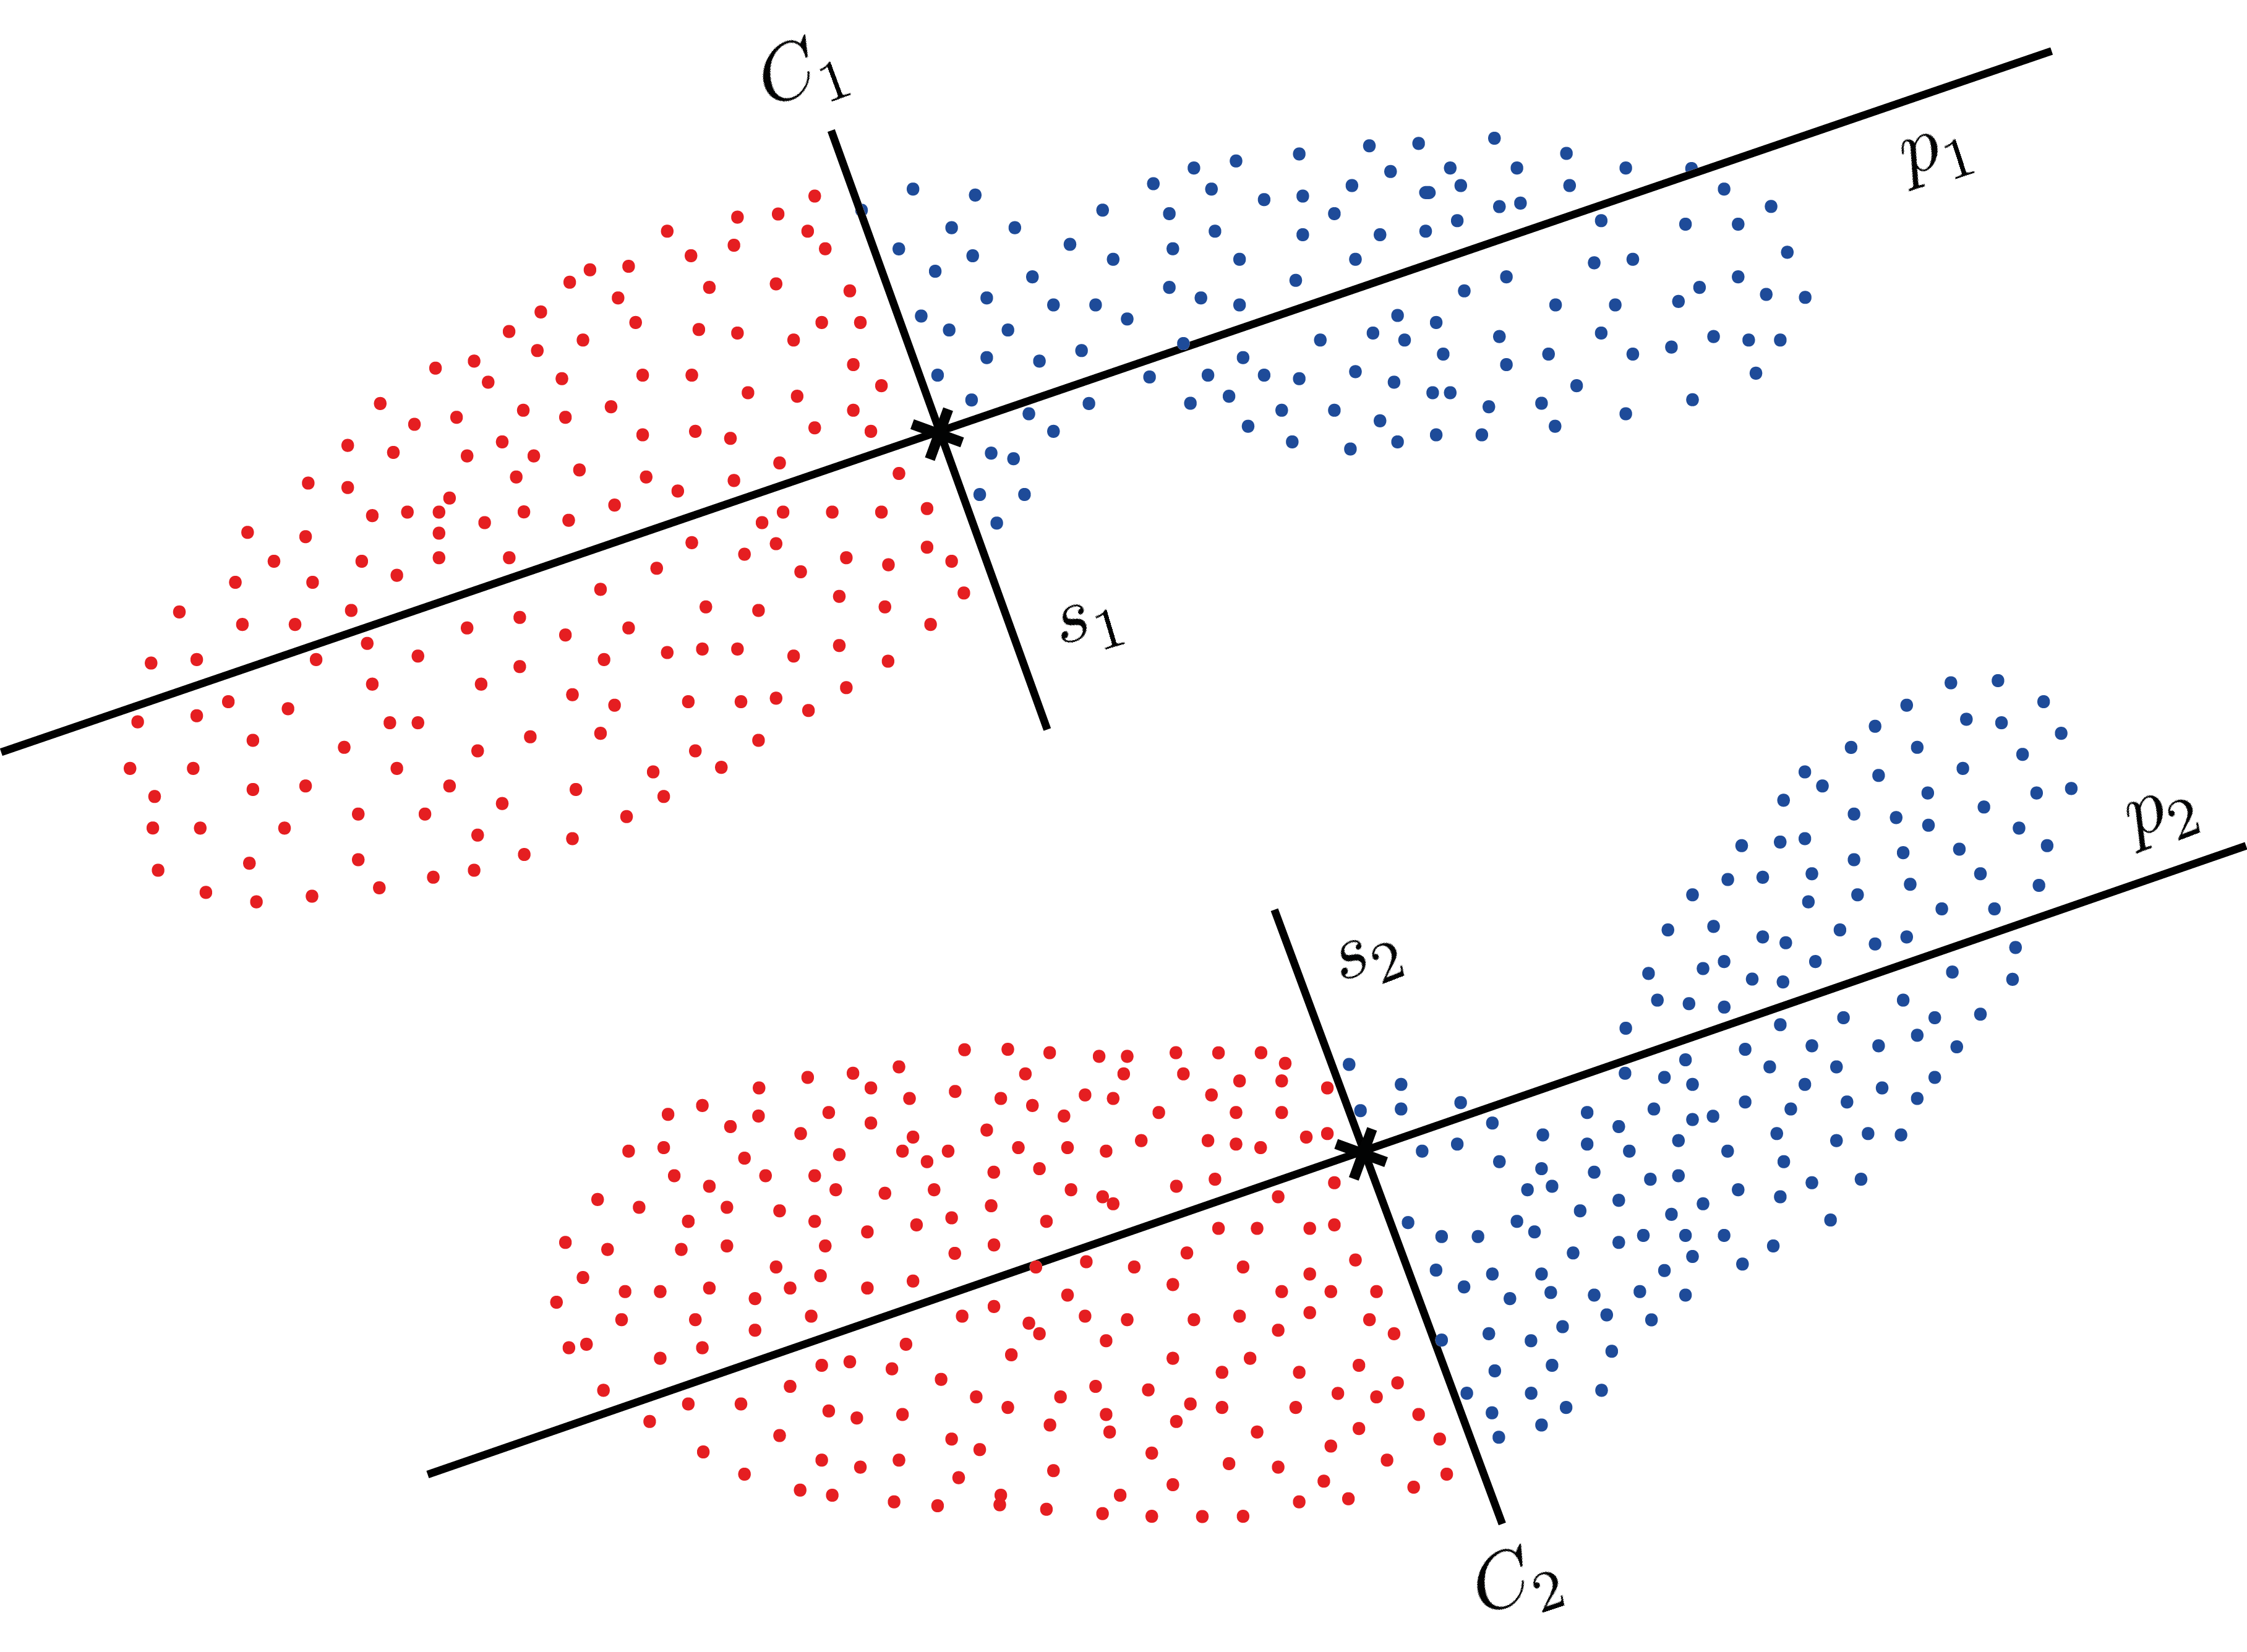
\includegraphics[width=0.7\linewidth]{illustration_axes}
 	\caption{General approach of the divide and conquer principle to segment a non-rigid object into its rigid parts}
 	\label{fig:dc_axes_2p}
 \end{figure}

 \begin{figure}
 	\centering
 	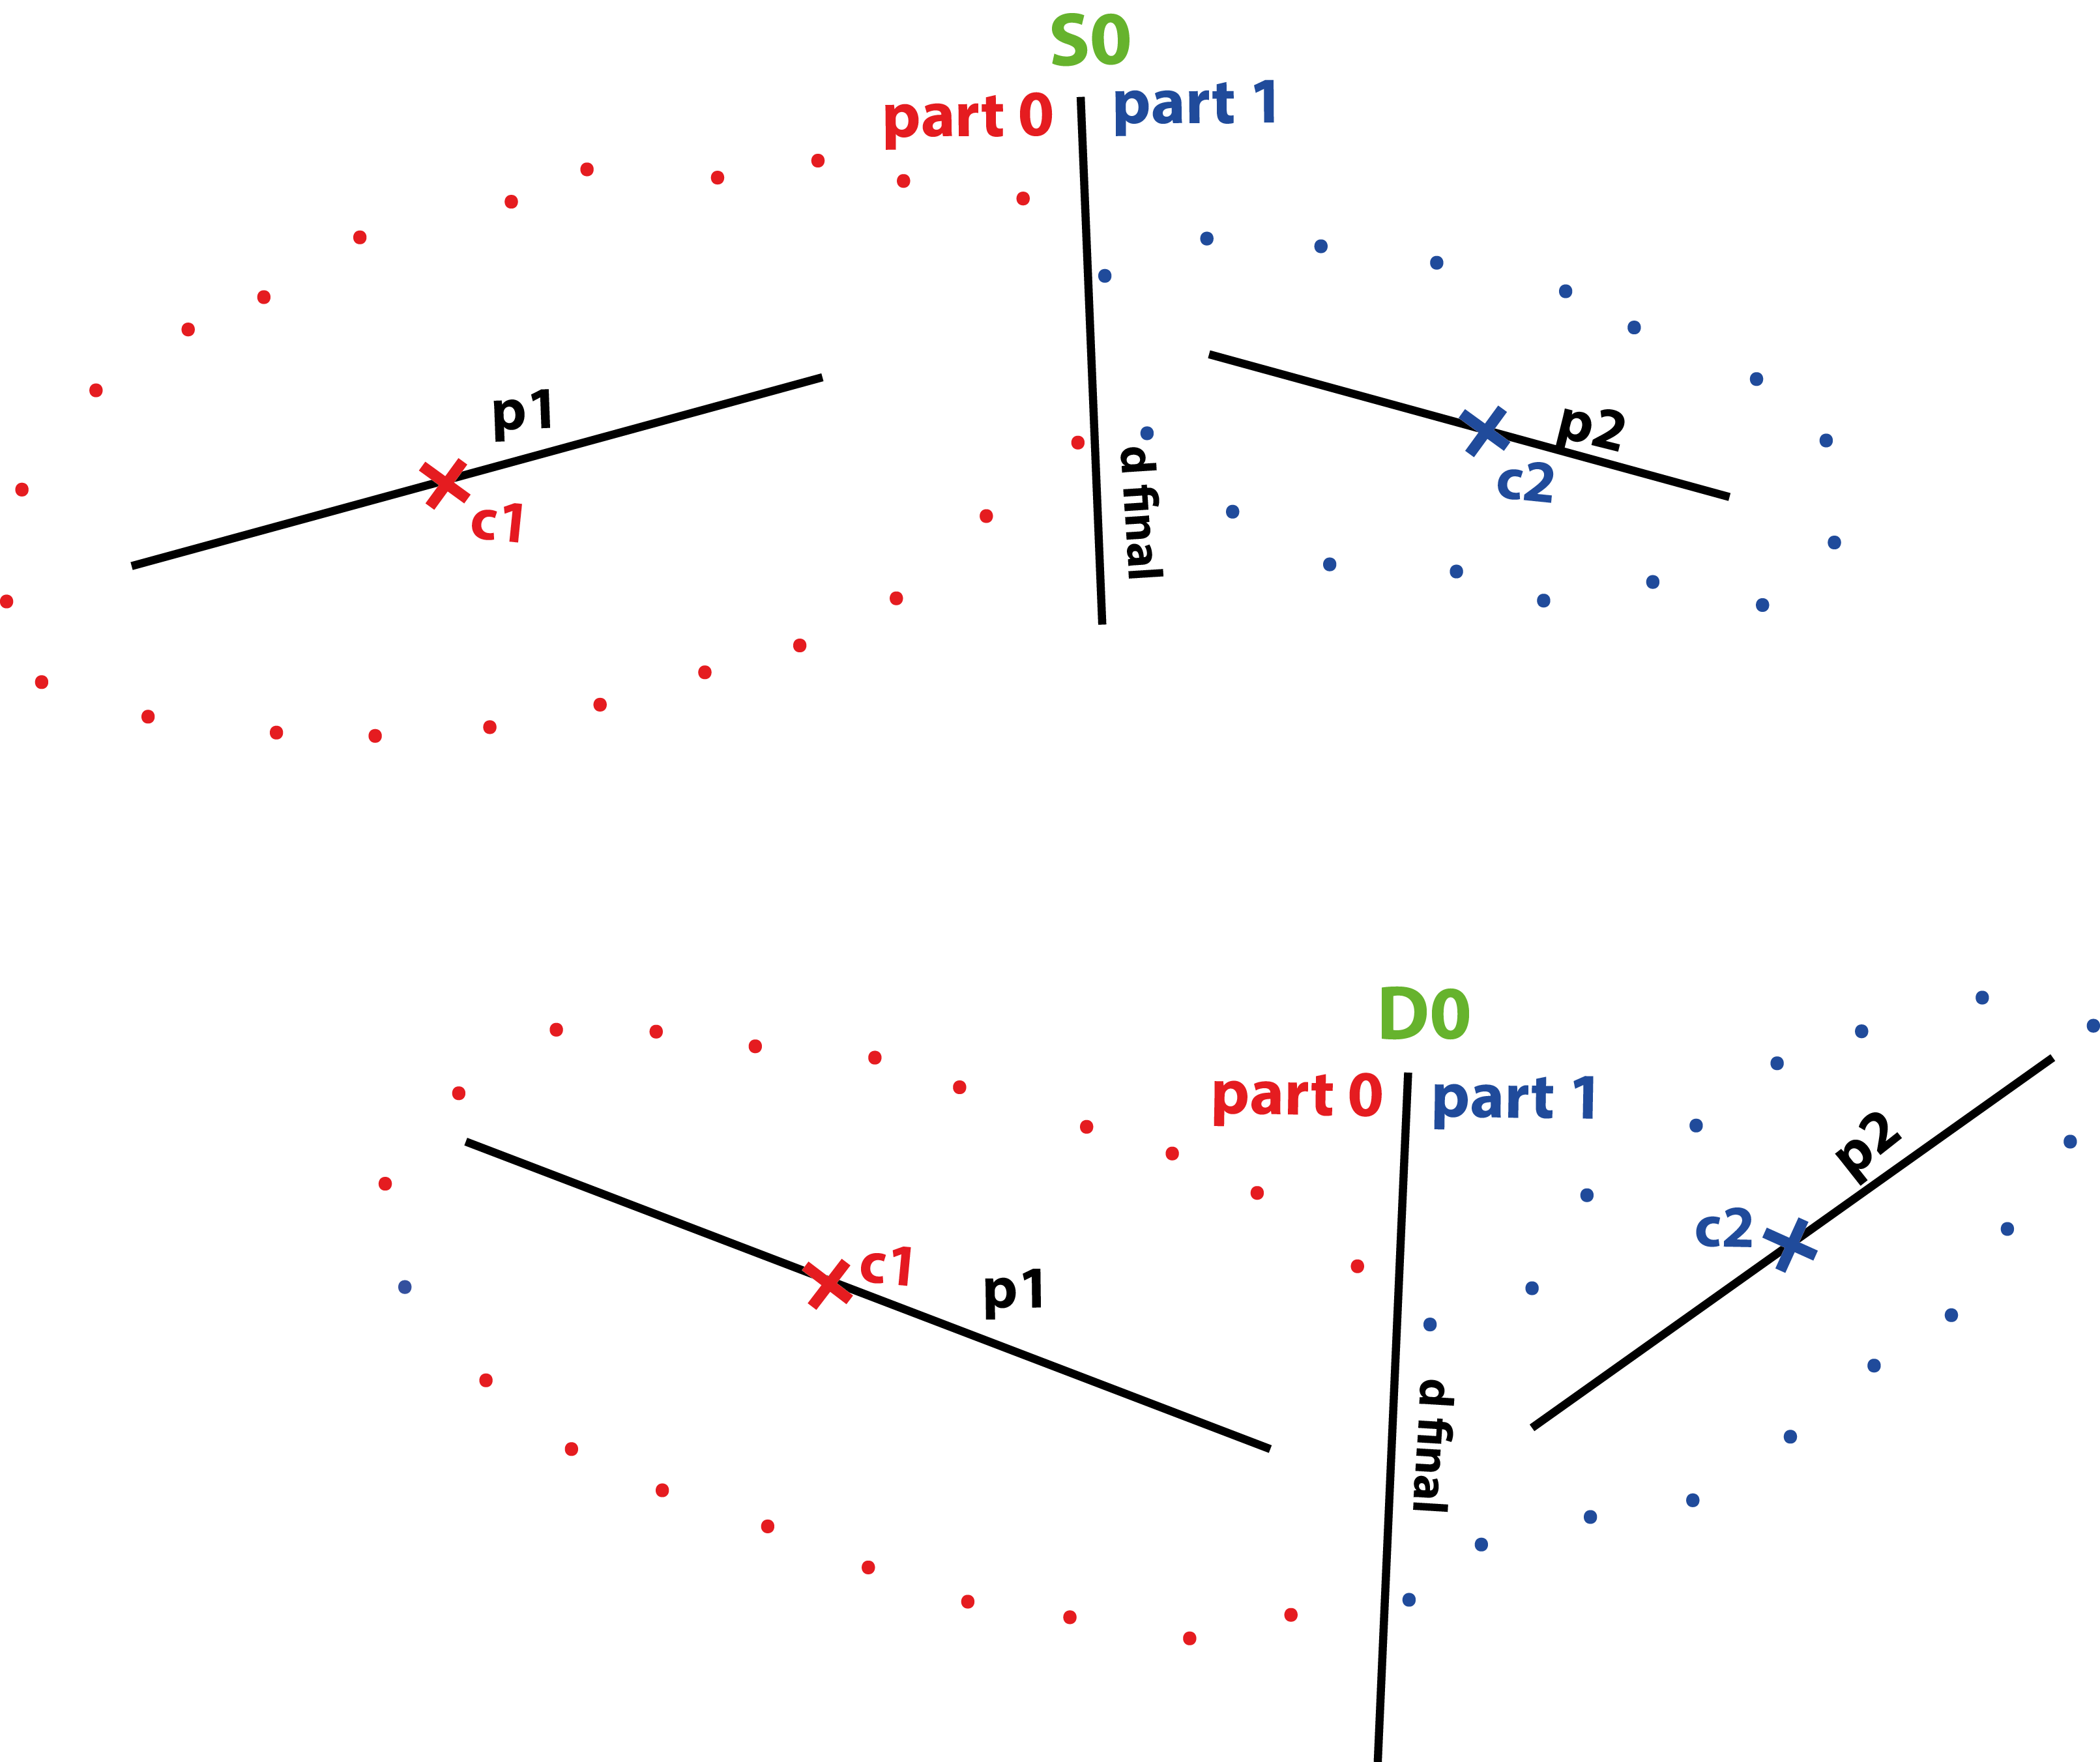
\includegraphics[width=0.7\linewidth]{illustration_results}
 	\caption{Resulting rigid parts (part0, part1) after termination of the iteration}
 	\label{fig:dc_results_2p}
 \end{figure}
 
 \subsection{Implementation Steps}
 
 \begin{enumerate}
 	\item The centroids \textit{c\textsubscript{S}} and \textit{c\textsubscript{D}} of \textit{S\textsubscript{0}} and \textit{D\textsubscript{0}} are computed.
 	
 	\item The principal axis \textit{p\textsubscript{S}} and \textit{p\textsubscript{D}}  are computed through \textit{c\textsubscript{S}} and \textit{c\textsubscript{D}} in order to orient the point clouds horizonally around their centroids.
 	
 	\item The secondary axis \textit{s\textsubscript{S}} and \textit{s\textsubscript{D}} perpendicular to \textit{p\textsubscript{S}} and \textit{p\textsubscript{D}} through \textit{c\textsubscript{S}} and \textit{c\textsubscript{D}} are computed.
 	
 	\item The dividers \textit{d\textsubscript{S}} and \textit{d\textsubscript{T}} to segment \textit{S\textsubscript{0}} and \textit{D\textsubscript{0}} into its assumed two rigid parts are initialized with the secondary axis \textit{s\textsubscript{S}} and \textit{s\textsubscript{D}}.
 	
 	\item The points \textit{P\textsubscript{0...N}} of \textit{S\textsubscript{0}}  are either allocated to \textit{S\textsubscript{left}} or \textit{S\textsubscript{right}} depending on its position to \textit{d\textsubscript{S}}. The same procedure is done with all points of \textit{D\textsubscript{0}}.
 	
 	\item ICP is computed between the rigid parts \textit{S\textsubscript{left}} and \textit{D\textsubscript{left}} as well as \textit{S\textsubscript{right}} and \textit{D\textsubscript{right}}.
 	
 	\item An error distance \textit{e\textsubscript{left}} and \textit{e\textsubscript{right}} is obtained. The part with the most error per point is assumed to be not rigid which gives back an indicator where to divide \textit{S\textsubscript{0}} and \textit{D\textsubscript{0}}.
 	
 	\item The dividers \textit{d\textsubscript{S}} and \textit{d\textsubscript{D}} are shifted to the direction of the highest error. To be continued from step 5 until the total error \textit{e\textsubscript{total}} doesn't get smaller.
 \end{enumerate}

\section{Segmentation of unknown number of rigid parts}

In case of having an unknown number of rigid parts \textit{n}, the algorithm above has to be applied recursively in order to find all part assignments \textit{P = \{{part\textsubscript{0} ... part\textsubscript{n}\}}}. \textit{S\textsubscript{0}} and \textit{D\textsubscript{0}} are thereby initially divided into two assumed rigid parts by the dividers \textit{d\textsubscript{S}} and \textit{d\textsubscript{D}} initialized with \textit{s\textsubscript{S}} and \textit{s\textsubscript{D}}. The goal is now to find single parts by sliding another divider over \textit{S\textsubscript{left}} and \textit{D\textsubscript{left}} as well as \textit{S\textsubscript{right}} and \textit{D\textsubscript{right}} until the error \textit{e} for one part doesn't get any smaller. The total error \textit{e\textsubscript{total}} is not used any more as dividing one part into two doesn't ensure that they are both rigid. After assigning points to a Part \textit{P} the geodesic distance between points of rigid parts can be used to find further connecting parts. By taking the dividers as joints and taking into account that rigid parts are located between the same joints, rigid parts in the middle of the object can be easier detected.

\subsection{Approach}

\subsection{Implementation Steps}

\subsection{Results}

\section{LRP as initial alignment}

Instead of cutting the object initially in half, as an initial step the largest rigid part is found and recursively from there all other linked parts can be detected.

\subsection{Overview}
As an initial step, the LRP algorithm tries to find the most reliable correspondences, the so-called largest rigid part (LRP), subsequently all other parts are detected that are linked to the LRP. The initial alignment stage tries to find sparse correspondences between two point clouds by applying a single rigid transformation to detect the largest subsets of points in two point clouds. Starting from the LRP all other parts are detected recursively.

\subsection{Algorithm} 

\subsubsection{Finding the LRP}

The algorithm also takes two point clouds \textit{S\textsubscript{0}} and \textit{T\textsubscript{0}} of the same object in different configurations as input.
The goal is to find a single rigid transformation \textit{T\textsubscript{init}} for all points of \textit{S\textsubscript{0}} to get potential corresponding points \textit{C\textsubscript{0} = \{(s\textsubscript{i}, t\textsubscript{j})\}} in \textit{T\textsubscript{0}}. For that, local descriptors of \textit{S\textsubscript{0}} and \textit{T\textsubscript{0}} are computed. The requirement for a sparse correspondance between two points \textit{s\textsubscript{i}} and \textit{t\textsubscript{j}}  is that they are \textit{reciprocal}, which means that the Euclidean distance \textit{d(s\textsubscript{i}, t\textsubscript{j})} between them is the smallest in both directions. Some of the sparse correspondances are asumed to be wrong. Therefore, RANSAC is used on the sparse correspondances \textit{C\textsubscript{0}} to estimate a rigid alignment that is supported by the largest number of points \textit{n} from \textit{S\textsubscript{0}} and \textit{T\textsubscript{0}}. To assign the LRP in \textit{S\textsubscript{0}} and \textit{T\textsubscript{0}}, the biggest point clusters \textit{C\textsubscript{s}} and \textit{C\textsubscript{t}} of the overlapping area \textit{G\textsubscript{s} = \{C\textsubscript{1}, ... , C\textsubscript{n}\} } and \textit{G\textsubscript{t} = \{C\textsubscript{1}, ... , C\textsubscript{n}\} } are detected. 


\subsubsection{Part discovery}

The remaining clusters from \textit{S\textsubscript{0}} and \textit{T\textsubscript{0}} that have not been registered yet are matched recursively by starting with clusters connected to already matched parts. First, all matched parts are excluded from the input point clouds  \textit{G\textsubscript{s(l+1)}} = \textit{S\textsubscript{0}} - \textit{C\textsubscript{sl}} and \textit{G\textsubscript{t(l+1)}} = \textit{T\textsubscript{0}} - \textit{C\textsubscript{tl}} defining \textit{l} as the number of already matched parts \{1, ..., n\}, \textit{C\textsubscript{sl}}. For that clusters are formed, using region taking into account that they are attached to already registered parts. The algorithm explained is applied until all body parts have been discovered.

\subsection{Steps}

\begin{enumerate}
	\item The centroids \textit{c\textsubscript{s}} and \textit{c\textsubscript{t}} of \textit{S\textsubscript{0}} and \textit{T\textsubscript{0}} are computed.
	
	\item The principal axis \textit{p\textsubscript{s}} and \textit{p\textsubscript{t}}  are computed through \textit{c\textsubscript{s}} and \textit{c\textsubscript{t}} in order to horizontally orient the objects around their centroids.
	
	\item The ICP is conducted as a first guess to find a transformation \textit{T\textsubscript{init}} for all points from \textit{S\textsubscript{0}} that results in the highest number of corresponding points \textit{n} in \textit{T\textsubscript{0}}, given the threshold \textit{T}.
	
	\item \textit{C\textsubscript{0}} contains the corresponding points from S\textsubscript{0} and T\textsubscript{0}, resulting from \textit{T\textsubscript{init}(S\textsubscript{0})}.
	
	\item The RANSAC approach is applied on \textit{C\textsubscript{0}} to find a  \textit{T\textsubscript{f}} that results in the highest number of corresponding points \textit{n} between \textit{T\textsubscript{f}(S\textsubscript{0})} and \textit{T\textsubscript{0}}.
	
	\item The LRP is assigned to \textit{C\textsubscript{s}} and \textit{C\textsubscript{t}} from the resulting point clusters \textit{G\textsubscript{s}} and \textit{G\textsubscript{t}}.
	
	\item Starting from parts that are connected to the LRP, corresponding points \textit{C\textsubscript{i}} for unmatched points from \textit{S\textsubscript{0}} and \textit{T\textsubscript{0}} are seeked. The clusters are given as a input from Step 5. 
		
\end{enumerate}

\section{Other approaches}

\section{Points-to-Ellipse fitting}

\subsection{Algorithm}

This algorithm only requires one point cloud containing \textit{m} points \{\textit{pt\textsubscript{0}, ..., pt\textsubscript{m}}\}. The basic idea is to segment the non-rigid object  \textit{S\textsubscript{0}} into its rigid parts \textit{part\textsubscript{1}} and {part\textsubscript{2}} by fitting ellipses to its rigid parts. 
\textit{S\textsubscript{0}} is divided perpendicular to its principal axis \textit{p\textsubscript{0}} into two assumed rigid parts \textit{S\textsubscript{left}} and \textit{S\textsubscript{right}}, initially defining the divider \textit{d} with the secondary axis \textit{s\textsubscript{0}}. The points of \textit{S\textsubscript{left}} and \textit{S\textsubscript{right}} are verified to 
form an ellipse by using its formular

\begin{equation}
\dfrac{x^2}{r_1^2} + \dfrac{y^2}{r_2^2} = 1
\end{equation}

Assuming to verify \textit{S\textsubscript{left}} forming an ellipse, \textit{r\textsubscript{1}} is half the length of the principal axis \textit{p\textsubscript{left}} of \textit{S\textsubscript{left}} through its centroid \textit{c\textsubscript{left}}. Furthermore, \textit{r\textsubscript{2}} is half the length of the secondary axis {s\textsubscript{left}} of \textit{S\textsubscript{left}}. Thereby, the centroid \textit{c\textsubscript{left}} needs to be located in the origin (0,0). 
Now, to check whether a point \textit{pt\textsubscript{i}} of \textit{S\textsubscript{left}} is located on the ellipse, the formular is remodeled and its x values is applied. 

\begin{equation}
(1 -  \dfrac{x^2}{r_1^2}) \cdot {r_2^2} = y^2
\end{equation}

The resulting y-value of the ellipse is compared to the points actual y-value. Given a certain threshold $\tau$ a point either accounts to the number of total points lying on the ellipse \textit{n}, or not.

\begin{equation}
n = \sum_{i=0}^{m}\begin{cases}1 \quad if \quad \|pt_i.y^2 - y^2 \| < \tau \\ 0 \quad otherwise\end{cases}
\end{equation}

The algorithm is repeated by sliding \textit{d} in the direction of the highest error \textit{e}. To be continued until the total error \textit{e\textsubscript{total} = e\textsubscript{left} + \textsubscript{right}} reaches its minimum.

\subsection{Steps}

\begin{enumerate}
	\item The centroid \textit{c\textsubscript{0}}  of \textit{S\textsubscript{0}} is computed.
	
	\item The principal axis \textit{p\textsubscript{0}} is computed through \textit{c\textsubscript{0}} and \textit{S\textsubscript{0}} horizontally oriented. 
	
	\item The secondary axis \textit{s\textsubscript{0}}  perpendicular to \textit{p\textsubscript{0}} through \textit{c\textsubscript{0}} is computed.
	
	\item The divider \textit{d} is initialized with the secondary axis \textit{s\textsubscript{0}} to segment \textit{S\textsubscript{0}} into two assumed rigid parts .
	
	\item The points of \textit{S\textsubscript{0}} are either allocated to \textit{S\textsubscript{left}} or \textit{S\textsubscript{right}} depending on its position to \textit{d\textsubscript{0}}.
	
	\item The ellipse formular is applied on \textit{S\textsubscript{left}} and \textit{S\textsubscript{right}}.
	
	\item An error \textit{e\textsubscript{left}} and \textit{e\textsubscript{right}} is obtained implying how many points of \textit{S\textsubscript{left}} and \textit{S\textsubscript{right}} form an ellipse. 
	
	\item The divider \textit{d} is shifted to the direction of the highest error. To be continued from step 5 until the total error \textit{e\textsubscript{total}} doesn't get smaller. 
\end{enumerate}

\subsection{Results}

\subsection{Reusing detected shapes}

After termination of the algorithm, one point cloud can be segmented into its rigid parts P \{part\textsubscript{1}, ..., part\textsubscript{n}\}. Their variables like the ellipses' centroid \textit{c\textsubscript{i}} and radii \textit{r\textsubscript{1}}, \textit{r\textsubscript{2}} can be used to segment similar point clouds in different configurations. As the shapes to be matched are already known, e.g. how they are linked, finding the position to be segmented is a lot easier.



\section{General Results}

\section{Improvements}

\section{Future work}

The approaches implemented in 2D are then implemented in 3D using the PCL. 

